\chapter{Kubernetes}

Kubernetes is one of the most widely used container orchestration tools. Many cloud platforms provide Kubernetes support. Many opponent container orchestration tools are built on top of Kubernetes.

\section{Kubernetes Basics}

\mync{Kubernetes}, also known as \mync{k8s}, is an open-source container orchestration system originally developed by Google. It automates the deployment, health screening and scaling of containers for containerized applications.

As an orchestration tool, Kubernetes mainly focuses on the following tasks:
\begin{itemize}
	\item Monitor the status of the containers, and restart / replace broken ones.
	\item Balance the load assigned to the containers.
	\item Strategically scale up and down the number of containers based on the total load.
\end{itemize}
From the above, Kubernetes can be seen as a more powerful practice of what docker compose tries to do. It comes with additional features such as the support on multi-server deployment.

Managed services such as ECS can also do container orchestration. However, these managed services are often proprietary and inclusive to a particular cloud service provider. With such proprietary services, it is difficult to migrate the applications across platforms or to local premises. Kubernetes, on the other hand, is open-source and platform-independent, hence would not pose that problem.

Nowadays, many cloud service providers also support Kubernetes-based container deployment solutions such as \myabb{Elastic Kubernetes Service}{EKS} by AWS and \myabb{Google Kubernetes Engine}{GKE} by Google Cloud. They are also managed services to some extend and each platform usually have some unique features, but in general the application can be migrated across platforms without too much difficulty.

\begin{shortbox}
	\Boxhead{Kubernetes and Docker Engine}
	
	Kubernetes was built on top of docker engine. It used a special program \verb|dockershim| to talk to the underlying docker engine. Recently, however, docker support has been deprecated in Kubernetes. Consequently, \verb|dockershim| has also been removed. Now Kubernetes directly talks with container runtimes.
\end{shortbox}


\subsection{Infrastructure}

Figure \ref{ch:vac:fig:kubernetescluster} demonstrates the key components Kubernetes has inside its cluster.
\begin{figure}[!htb]
	\centering
	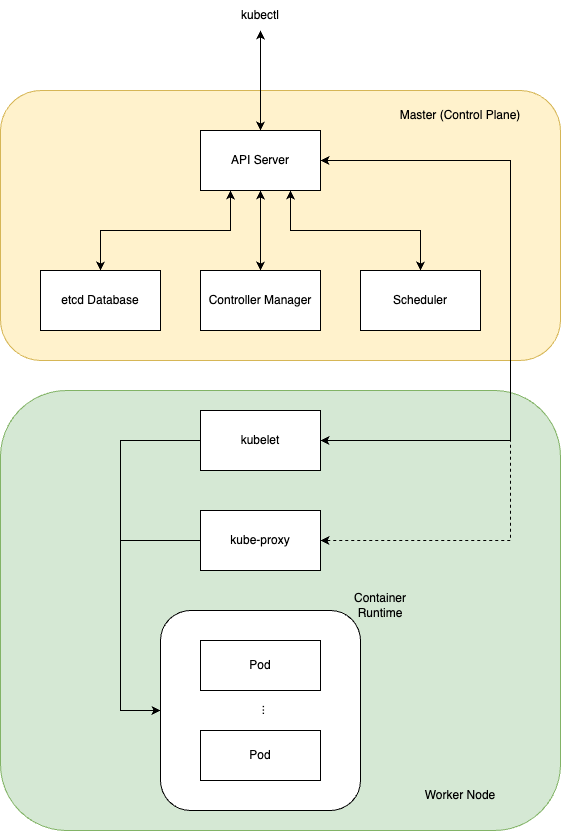
\includegraphics[width=250pt]{chapters/part-3/figures/k8sarchitecture.png}
	\caption{Kubernetes cluster and its key components.} \label{ch:vac:fig:kubernetescluster}
\end{figure}
As shown in Fig. \ref{ch:vac:fig:kubernetescluster}, Kubernetes manages containers in a centralized ``master-worker'' manner, where the \mync{master node} (also known as \mync{control plane}) in yellow interacts with the user and schedules the Pods to be deployed for each work node. The \mync{work nodes} (also known as \textbf{nodes}, for short) in green, on the other hand, process the application data. The arrows in Fig. \ref{ch:vac:fig:kubernetescluster} represents the control flow. Notice that the application data flows differently and it does not pass through the master. There can be multiple master nodes (in replica mode) and worker nodes, though only one of each is shown in Fig. \ref{ch:vac:fig:kubernetescluster}.

Key components in the master and the nodes and their functions are summarized in Table \ref{ch:vac:tab:keycomponents}.

\begin{table}[!htb]
	\centering
	\caption{Key components in Kubernetes master and nodes.} \label{ch:vac:tab:keycomponents}
	\begin{tabularx}{\textwidth}{llX}
		\hline
		Component & Location & Description \\
		\hline
		\verb|etcd| & Master & A distributed key-value pair database that stores the status of the Kubernetes cluster. The consistency of the distributed database is achieved based on Raft consensus algorithm. \\ \hline
		API server & Master & The gateway to handle all interactions with the Kubernetes cluster. For example, \verb|kubectl| requests from the user are handled by API server. \\ \hline
		Scheduler & Master & The optimizer that calculates the desired Pod distributions among all nodes based on the total load and the hardware limits. Notice that scheduler is not involved into load balance directly. A separate load balancer service can be created to actually direct the traffic. \\ \hline
		Controller Manager & Master & A set of controllers or control functions to reconcile the actual Kubernetes cluster status with what has been calculated by the scheduler and stored in \verb|etcd|. \\ \hline
		Kubelet & Node & Local controller for the node. It ensures that all the Pods assigned to the node are running, and it keeps listening to the master for further instructions. \\ \hline
		Kube Proxy & Node & The internet service provider in the node. \\
		\hline
	\end{tabularx}
\end{table}

Each node can host multiple Pods. A Pod object is a single container or a collection of containers for a single task, and it is also the smallest unit that Kubernetes controls directly. Notice that in Kubernetes, containers never run directly in a node. They are always grouped into Pods. More details about the Pod object are introduced in later Section \ref{ch:vac:sec:objects}.

Both master and nodes can run on multiple servers or VMs. For master, multiple master replicas can run in parallel to take care of user requests and provide database services. The ``decision makers'', i.e. the controller manager and scheduler, run only on one of the master nodes which is elected via a leader election process. Should the decision maker master fail, one of the replicas will be promoted. For nodes, multiple nodes can run together to precess information in parallel and Kubernetes manages the distribution of load among them.

It is worth mentioning that many services cluster-level services such as ClusterIP, NodePort, LoadBalancer and Ingress Controllers, though being cluster-level, run in worker nodes but not in the master. 

\subsection{Installation}

Kubernetes is not a single piece of software but more an architecture that involves many pieces of software such as:
\begin{itemize}
  \item \verb|kubectl| the CLI
  \item \verb|kube-apiserver| the API server
  \item \verb|etcd| the distributed key-value pair database
  \item \verb|kube-scheduler| the scheduler
  \item \verb|kube-controller-manager| the control manager
  \item Kubelet
  \item Kube Proxy
  \item Kubernetes-supported container runtime such as \verb|containerd|
  \item Container Network Interface (CNI) plugin such as Calico
  \item \ldots
\end{itemize}
The installation guidance of Kubernetes can be found at its official website \textit{kubernetes.io}. In a production environment, the administrator shall install and configure the above tools on the servers by himself. This gives him the flexibility of customizing the tools. However, the process can be tedious and requires experience.

In this notebook, for demonstration purpose, we will use Minikube to help build a Kubernetes cluster. Minikube is an open-source software developed by the Kubernetes community to start a VM and run a single-node Kubernetes cluster on a local machine. It automates most of the tools installations and configurations which is in favour of the scope of this notebook. 

We still need to install Minikube and also \verb|kubectl|. As introduced earlier, \verb|kubectl| is used to interact with Kubernetes clusters deployed either locally or remotely. It is always recommended to have \verb|kubectl| installed on the local machine wherever the Kubernetes cluster is deployed. The installation of \verb|kubectl| can be found at Kubernetes website at
\begin{lstlisting}
https://kubernetes.io/docs/tasks/tools/install-kubectl-linux/
\end{lstlisting}
Minikube installation can be found at
\begin{lstlisting}
https://minikube.sigs.k8s.io/docs/start/
\end{lstlisting}

Once Minikube is installed, start it using
\begin{lstlisting}
$ minikube start
\end{lstlisting}
When starting Minikube, it automatically detects which container engine to use, and some configurations might be required subsequently.

When running Minikube, it uses existing VM engines such as VirtualBox, or container engines such as docker and podman installed on the local machine to start a VM or container that hosts Kubernetes. Therefore, it will need to execute the VM tools or the container engines. In naive RHEL, Minikube needs to execute podman. Some of the commands Minikube need to run require sudo privilege, and as a result, it requires \verb|NOPASSWD| configuration to start the Kubernetes cluster correctly. 

This can be done as follows. Open the sudoer configuration file by
\begin{lstlisting}
$ sudo visudo
\end{lstlisting}
and append
\begin{lstlisting}
<user name> ALL=(ALL) NOPASSWD: /usr/bin/podman
\end{lstlisting}
to the file.

Once Minikube is started, \verb|kubectl| installed on the local machine should be able to detect the Kubernetes running inside. Sse the following command to verify that \verb|kubectl| has detected and connected with the Kubernetes runtime.
\begin{lstlisting}
$ kubectl cluster-info
Kubernetes control plane is running at https://192.168.49.2:8443
CoreDNS is running at https://192.168.49.2:8443/api/v1/namespaces/kube-system/services/kube-dns:dns/proxy
\end{lstlisting}

\begin{shortbox}
\Boxhead{Minikube's Built-in \texttt{kubectl}}

Minikube also comes with a built-in \verb|kubectl|. It is possible to use that \verb|kubectl| instead of installing one separately. To very the existence of the built-in \verb|kubectl|, start Minikube first and then use

\begin{lstlisting}
$ minikube kubectl -- cluster-info
Kubernetes control plane is running at https://192.168.49.2:8443
CoreDNS is running at https://192.168.49.2:8443/api/v1/namespaces/kube-system/services/kube-dns:dns/proxy
\end{lstlisting}
where \verb|--| in the command tells the shell that all the followed arguments shall be passed to \verb|kubectl| inside Minikube, but not \verb|minikube| itself. For convenience, one may want to use alias as follows
\begin{lstlisting}
$ alias kubectl="minikube kubectl --"
\end{lstlisting}

With the above been said, it is still recommended that \verb|kubectl| to be installed on the local machine, not just in the VM. 
\end{shortbox}

It is possible to run Kubernetes cluster directly on a host machine OS without VM if that machine is running Linux. However, this is not recommended for reasons pertaining to access control, security, and isolation. It is generally a better practice to deploy Kubernetes clusters in VMs.

The configuration file for \verb|kubectl| is usually located at \verb|~/.kube/config|. It determines the basic setups of the \verb|kubectl| instance, such as which Kubernetes cluster \verb|kubectl| communicates with.

\subsection{Kubernetes Cluster Manipulation}

There are at least two ways for a user to interact with a Kubernetes cluster and deploy or manipulate services in it.
\begin{itemize}
  \item Imperative approach: use \verb|kubectl| commands to directly start, change or stop Pods and services.
  \item Declarative approach: prepare Kubernetes configuration files that describes the ``desired state'' of the Kubernetes cluster, and use \verb|kubectl -f| command to implement the files. Kubernetes decides how to deploy Pods on servers to achieve the desired state.
\end{itemize}
Both approaches are introduced as follows. 

\vspace{0.1in}
\noindent \textbf{Cluster Deployment with Imperative Approach}
\vspace{0.1in}

The imperative approach, in some sense, destroys the purpose of Kubernetes as a container orchestration tool since the user decides the deployment of Pods and services manually. On the other hand, the declarative approach takes advantage of the full capability of Kubernetes and it is usually considered a better practice. Yet, learning the imperative approach helps the user with getting familiar with \verb|kubectl| commands. In this section, imperative approach and its relevant generally used \verb|kubectl| commands are briefly introduced.

Use the following to view the entire list of \verb|kubectl| supported commands.
\begin{lstlisting}
$ kubectl help
kubectl controls the Kubernetes cluster manager.

 Find more information at: https://kubernetes.io/docs/reference/kubectl/

Basic Commands (Beginner):
  create          Create a resource from a file or from stdin
  expose          Take a replication controller, service, deployment or pod and expose it as a new Kubernetes service
  run             Run a particular image on the cluster
  set             Set specific features on objects

Basic Commands (Intermediate):
  explain         Get documentation for a resource
  get             Display one or many resources
  edit            Edit a resource on the server
  delete          Delete resources by file names, stdin, resources and names, or by resources and label selector

Deploy Commands:
  rollout         Manage the rollout of a resource
  scale           Set a new size for a deployment, replica set, or replication controller
  autoscale       Auto-scale a deployment, replica set, stateful set, or replication controller

Cluster Management Commands:
  certificate     Modify certificate resources
  cluster-info    Display cluster information
  top             Display resource (CPU/memory) usage
  cordon          Mark node as unschedulable
  uncordon        Mark node as schedulable
  drain           Drain node in preparation for maintenance
  taint           Update the taints on one or more nodes

Troubleshooting and Debugging Commands:
  describe        Show details of a specific resource or group of resources
  logs            Print the logs for a container in a pod
  attach          Attach to a running container
  exec            Execute a command in a container
  port-forward    Forward one or more local ports to a pod
  proxy           Run a proxy to the Kubernetes API server
  cp              Copy files and directories to and from containers
  auth            Inspect authorization
  debug           Create debugging sessions for troubleshooting workloads and nodes
  events          List events

Advanced Commands:
  diff            Diff the live version against a would-be applied version
  apply           Apply a configuration to a resource by file name or stdin
  patch           Update fields of a resource
  replace         Replace a resource by file name or stdin
  wait            Experimental: Wait for a specific condition on one or many resources
  kustomize       Build a kustomization target from a directory or URL

Settings Commands:
  label           Update the labels on a resource
  annotate        Update the annotations on a resource
  completion      Output shell completion code for the specified shell (bash, zsh, fish, or powershell)

Subcommands provided by plugins:

Other Commands:
  api-resources   Print the supported API resources on the server
  api-versions    Print the supported API versions on the server, in the form of "group/version"
  config          Modify kubeconfig files
  plugin          Provides utilities for interacting with plugins
  version         Print the client and server version information

Usage:
  kubectl [flags] [options]
\end{lstlisting}

Use
\begin{lstlisting}
$ kubectl create <object type> <object name> --<argument>
\end{lstlisting}
to create and deploy an object, and use
\begin{lstlisting}
$ kubectl get <object type>
\end{lstlisting}
to view deployed objects of certain type. Notice that in \verb|kubectl get| is usually followed by the plural form of the object type. An example is given below.
\begin{lstlisting}
$ kubectl create deployment <deployment name> --image=<image name>
$ kubectl get deployments
\end{lstlisting}
Deployment object is deployed in the above example. More about Deployment object will be given in later Section \ref{ch:vac:sec:objects}. It is one of the most commonly used Kubernetes objects and serves well as an example to illustrate imperative approach. Notice that the image assigned to the deployment, in the above example \texttt{hello-world}, needs to be reachable by Kubernetes. In this example, the image is to be deployed by the Kubernetes cluster deployed in the Minikube environment, and hence any image locally built in the host machine will not be reachable. The image has to be stored on an online registry.

The deployed Pods will be default have a cluster-level internal IP. There are the following problems with this internal IP: it is dynamic, and it is not accessible from outside the cluster. To expose the IP and port, a separate Service object needs to be used as follows.
\begin{lstlisting}
$ kubectl expose deployment <deployment name> --type=<service type>
\end{lstlisting}
where Service object type can be \verb|ClusterIP|, \verb|NodePort|, \verb|LoadBalancer|, etc. More about Service object will be given in later Section \ref{ch:vac:sec:objects}.

To scale up and down the number of Pods in a Deployment object, use
\begin{lstlisting}
$ kubectl scale --replicas=<number> deployment <deployment name>
\end{lstlisting}

And finally to update the image of the deployment, use
\begin{lstlisting}
$ kubectl set image deployment/<deployment name> <container name>=<image name: tag>
\end{lstlisting}
For example,
\begin{lstlisting}
$ kubectl set image deployment/nginx-deployment my-nginx-container=nginx:1.25.1
\end{lstlisting}

The user can check the status of the roll out by
\begin{lstlisting}
$ kubectl rollout status deployment/<deployment name>
\end{lstlisting}
When Kubernetes is rolling out a new version, the old version will not be shutdown. This minimizes the blackout time when an application is being updated.

The user can check the history of the roll out using
\begin{lstlisting}
$ kubectl rollout history deployment/<deployment name> [--revision=<revision index>]
\end{lstlisting}
where \verb|[--rivision]| will provides details to the roll out.

To roll back to an earlier version in the history, use
\begin{lstlisting}
$ kubectl rollout undo deployment/<deployment name> [--to-revision=<revision index>]
\end{lstlisting}
where if \verb|--to-revision| is not used, the command rolls back to the earlier latest version.

\vspace{0.1in}
\noindent \textbf{Cluster Deployment with Declarative Approach}
\vspace{0.1in}

Kubernetes configuration files describe the desired final status of the Kubernetes cluster. Should these files be passed to Kubernetes, it should be able to determine the processes to deploy relevant Kubernetes objects and eventually realize and maintain the desired state. This is known as the declarative approach and it is the default and recommended way Kubernetes shall be used. The declarative approach has at least the following advantages over the imperative approach:
\begin{itemize}
  \item It automates the Kubernetes deploying by using configuration files instead of the user running \verb|kubectl| commands manually, which simplifies the process and reduces human error.
  \item It leverages on the container orchestration capability of Kubernetes.
\end{itemize}
These advantages are critical especially in large-scale projects when there are multiple Kubernetes objects in the cluster.

The details of Kubernetes objects are introduced in later Section \ref{ch:vac:sec:objects}. In this section, a simple example is used to illustrate the basic commands for the declarative approach. Below is an example from the Kubernetes website. It contains the configuration of two objects.
\begin{lstlisting}
apiVersion: apps/v1
kind: Deployment
metadata:
  name: nginx-deployment
  labels:
    app: nginx
spec:
  replicas: 3
  selector:
    matchLabels:
      app: nginx
  template:
    metadata:
      labels:
        app: nginx
    spec:
      containers:
      - name: nginx
        image: nginx:1.14.2
        ports:
        - containerPort: 80
\end{lstlisting}

Some commonly used fields used in the Kubernetes configuration files are briefly summarized below.
\begin{itemize}
	\item \verb|apiVersion|: The API version of the object. Different object types are supported in different API versions.
	\item \verb|kind|: The object type.
	\item \verb|metadata|: The name and labels of the object. 
	\item \verb|spec|: The specifications of the object. Different object types require different specifications.
\end{itemize}
More details of the configuration file composing of each type of Kubernetes object are introduced in later Section \ref{ch:vac:sec:objects}. 

With the image and the configuration files ready, the next step is to deploy the nodes, Pods, and containers. The \verb|kubectl| CLI is used to instruct Kubernetes to deploy the objects as follows.
\begin{lstlisting}
$ kubectl apply -f <configuration file> / <files directory>
\end{lstlisting}
This essentially asks the master node in the Kubernetes cluster to start taking actions following the Kubernetes configuration files, such as to inform the nodes to start creating Pods and containers. The master node also keeps monitoring the status of each work node, to make sure that everything is running as planned. If there is a container failure, etc., the master node will guide the associated note to restart the container.

It is possible to consolidate the configuration files of objects into one configuration file. To do that, use \verb|---| to split the configurations for each object in the conjunctive configuration file as follows. It is of personal preference whether to use conjunctive configuration files or separate configuration files for all objects.
\begin{lstlisting}
<configurations for object 1>
---
<configurations for object 2>
---
<...>
\end{lstlisting}
The order of the configurations appears in the file usually does not matter. However, it is often considered a better practice to put cluster-level objects such as Service objects in front of work split objects such as Development objects.

With the help of Kubernetes declarative approach, it is possible to update the cluster simply by revising the configuration files, and pass them to Kubernetes as if the cluster is to be deployed for the first time. Kubernetes automatically checks revised configuration files, comparing them with existing running objects, and update them if necessary.

It is recommended to check the status of the Pods using \verb|kubectl get pods| once the cluster is updated. After the update, the Pods should be restarted, and hence the ``RESTARTS'' tag shall increase. To ensure that the update is successful, use \verb|kubectl describe| to check the details of the relevant objects.

Notice that there is a limitation on what can be updated to an existing Kubernetes deployment. For an existing object, only certain fields in the Kubernetes configuration files are allowed to be revised. For example, for a Pod, the image can be changed while the ports cannot. Some objects types are more flexible than others when comes to object updating. The user shall choose wisely what object types to use considering what updates need to be made in future.

To revert what has been applied in a Kubernetes configuration file, use
\begin{lstlisting}
$ kubectl delete -f <configuration file>
\end{lstlisting}
The user can also delete certain types of objects by labels by
\begin{lstlisting}
$ kubectl delete <object type 1>[, <object type 2>, ...] -l <label>
\end{lstlisting}

\vspace{0.1in}
\noindent \textbf{Kubernetes Cluster Status Check}
\vspace{0.1in}

To retrieve the status of a group of objects, use
\begin{lstlisting}
$ kubectl get <object type>
\end{lstlisting}
where \verb|<object type>| can be \verb|pods|, \verb|services|, etc. For more details of a specific object, use
\begin{lstlisting}
$ kubectl describe <object type> <object name>
\end{lstlisting}
for example, to check the containers running in a Pod. If \verb|<object name>| is neglected, Kubernetes returns detailed information of all objects of the given object type. For a running object, use
\begin{lstlisting}
$ kubectl logs <object name>
\end{lstlisting}
to check the log file of that object.

Minikube provides a web-based dashboard where the user can conveniently check the status of the cluster. Use
\begin{lstlisting}
$ minikube dashboard
\end{lstlisting} 
to start the dashboard and follow the instructions on the concole to open the dashboard. The dashboard gives the detailed information of running objects in the Kubernetes cluster, such as the healthy status of Pods, the cluster-level internal IP of objects, etc.


Kubernetes treats the above as an update and will action accordingly.

\section{Basic Kubernetes Objects} \label{ch:vac:sec:objects}

Kubernetes supports a long list of objects, and the list is growing along with Kubernetes version. The list can be displayed by
\begin{lstlisting}
$ kubectl api-resources
\end{lstlisting}

It is hardly possible to cover all the Kubernetes objects in this notebook. This section only introduces the commonly used basic Kubernetes objects summarized in Table \ref{ch:vac:tab:objtype}.
\begin{table}[!htb]
	\centering
	\caption{Commonly used Kubernetes object types.} \label{ch:vac:tab:objtype}
	\begin{tabularx}{\textwidth}{lX}
		\hline
		Object Type & Description \\
		\hline
		Pod & Represents a single instance of a process running in the cluster. A Pod contains one or multiple containers that work closely to deliver a basic function. It is the smallest unit of process in Kubernetes. \\ \hline
		Deployment & Manages the deployment and scaling of a set of identical Pods, ensuring the desired number of replicas are running and providing rolling updates for seamless application upgrades. \\ \hline
		Service & Enables network access to the node or to a set of Pods using a stable IP address and DNS name. It provides load balancing across multiple Pod replicas and allows external traffic to be directed to the appropriate Pods. \\ \hline
		ConfigMap & Stores configuration data in key-value pairs, which can be consumed by Pods as environment variables, command-line arguments, or mounted as files. \\ \hline
		Volume & Provides a way to provision and manage persistent storage resources in a cluster. \\
		\hline
	\end{tabularx}
\end{table}

\subsection{Pod Object}

\mync{Pod} object is the smallest and most fundamental unit in a node that Kubernetes interacts with. A Pod is essentially a ``wrap'' that hosts one or multiple containers that work closely with each other. Pod contains shared resources such as volumes for all the containers it hosts. The containers in a Pod can also communicate each other via \verb|localhost|. A Pod has a cluster-internal IP by default.

Just like a container, Pods are designed to be ephemeral. Kubernetes can start and stop them depending on the load and the traffic coming into the cluster, and when they are removed, their data vanishes. Of course there are many ways to persist the data, for example by directing the data into a volume or a database.

The user can deploy Pods using either \verb|kubectl| command imperatively or in Kubernetes configuration files declaratively. However, the user would not do so in practice, as it destroys the purpose of using Kubernetes.

A Pod is assigned with a cluster-level internal IP by default, and that IP can be used for communications inside the Kubernetes cluster. It has the following problems though, making the IP address difficult to use:
\begin{itemize}
  \item The IP address is internal the cluster, hence useless to entities outside the container.
  \item Even for communications inside the cluster, the IP address is not convenient to use since it is dynamic.
\end{itemize}

\subsection{Deployment Object}

It is more often that the user would want to deploy Deployment objects instead of Pods. A \mync{Deployment} object serves as the ``controller'' of one or a group of identical Pods, and it serves as a good example to illustrate declarative approach where the user specifies a desired state and the Deployment object carries out the necessary procedures to realize that state. A Deployment object can do at least the following for the Pods it manages:
\begin{itemize}
  \item Start and stop the Pods strategically at different word nodes.
  \item Monitor the healthy status of the Pods and strategically restart them when necessary.
  \item Scale up and down the number of Pods.
  \item Balance the loads that go into each Pod.
  \item Update or roll back the Pods.
\end{itemize}

As an example, a Kubernetes cluster file that deploys an Deployment object is given below. Notice that Deployment object is supported in API version \verb|apps/v1|.
\begin{lstlisting}
apiVersion: apps/v1
kind: Deployment
metadata:
  name: nginx-deployment
  labels:
    app: nginx
spec:
  replicas: 3
  selector:
    matchLabels:
      app: nginx
  template:
    metadata:
      labels:
        app: nginx
    spec:
      containers:
        - name: nginx
          image: nginx
          ports:
            - containerPort: 80
\end{lstlisting}
Some highlights under \verb|spec| are introduced below.
\begin{itemize}
	\item \verb|replicas|: the number of Pods under the Deployment object should maintain. The value can be zero if no Pods need to be deployed initially.
	\item \verb|selector.matchLabels|: a set of labels, which if a Pod possesses, will be monitored and likely managed by the Deployment object.
	\item \verb|template|: the template that describes the Pods this Deployment object creates, including:
    \begin{itemize}
      \item \verb|metadata.labels|: the labels the Pods will inherit.
      \item \verb|spec.containers|: the containers details, such as name, image, port, etc.
    \end{itemize}
\end{itemize}
Notice that a Deployment object can deploy only identical Pods from the same template. If different types of Pods need to be deployed, different Deployment objects are required. However, under one Pod, there can be multiple containers populated from different images. Notice that \texttt{template.spec.containers} contains a list of containers, each with its name, image, ports, etc. Append that list if multiple containers are required under the same Pod.

An alternative to \texttt{selector.matchLabels} is \texttt{selector.matchExpressions}, the later of which provides a more powerful and flexible way of mapping labels. More details of \texttt{selector.matchExpressions} is not introduced in this notebook, as \texttt{selector.matchLabels} should serve well in most scenarios.

\begin{shortbox}
\Boxhead{Labels in \texttt{selector} and \texttt{template}}

It may feel redundant that the same labels appear twice under both \texttt{selector.matchLabels} and \texttt{template.metadata.labels}. This sense of redundancy often stems from the assumption that a Deployment object should watch (and only watch) the Pods it creates.

In reality, multiple controllers can ``monitor'' the same Pods, potentially for metrics, auditing, or other read-only operations. A Pod has exactly one owner which is the controller that creates the Pod, but it can be monitored by other controllers or tools via label selector.

By splitting \texttt{selector.matchLabels} and \texttt{template.metadata.labels} instead of automatically inheriting one from the other, Kubernetes provides flexibility in how Pods and Deployment objects are architected. Additional labels can be added in the template to support other purposes—like monitoring, cost allocation or environment tagging without affecting the Deployment’s fundamental ownership of those Pods.

\end{shortbox}

When a new version of an image becomes available, we may want to update the containers accordingly. Re-apply the same configuration file would not help, as Kubernetes would reject apply request if no change is detected in the configuration file. It would not check whether the image is in its latest version. The following imperative command which has been introduced earlier can be used to update the image.
\begin{lstlisting}
$ kubectl set image deployment/<deployment name> <container name>=<image name: tag>
\end{lstlisting}
The image in the specified container will be updated. Notice that the new image will be downloaded only if it has a different tag. This encourages the developer to update the tag formally when publishing images.

Some optional yet useful configurations that Deployment object supports are briefly introduced as follows.

The \verb|livenessProbe| under \verb|spec.containers| of Deployment objects allows the user to define how the healthiness of the container shall be monitored. For example, the user can define a watch dog by asking the container to send an HTTP get request to certain port at certain frequency, and so on. Notice that Kubernetes has default liveness probe mechanism. Still, the flexibility where the user can override it with a custom probe is appreciated.

By default, the Deployment object will pull the images when
\begin{itemize}
  \item The image is not saved in the locally, in which case Kubernetes has to pull the image.
  \item The \verb|:latest| tag is used with the image, in which case Kubernetes will pull the image each time before launching the containers.
\end{itemize}
The \texttt{spec.containers.imagePullPolicy} of Deployment objects can be used to change the policy of pulling the image. For example, if \texttt{imagePullPolicy: Always} is used, the Deployment project will always pull the image before starting the containers.

\subsection{Service Object} \label{ch:vac:subsec:k8snetworking}

A \mync{Service} object is used to build network services in a Kubernetes cluster. As introduced earlier, though objects such as Pods will be automatically assigned with cluster-level internal IPs, they are close to useless in practice. Service objects can be used to build a more useful and robust network infrastructure for a Kubernetes cluster.

There are 4 subtypes of Service objects, including
\begin{itemize}
	\item ClusterIP: a ClusterIP Service object is assigned with a static cluster-level internal IP which is useful for communications of services within the cluster.
	\item NodePort: a NodePort Service object exposes a port on all the work nodes, using which outside entities can communicate with the NodePort Service object and then talk to objects inside the Kubernetes cluster. Notice that NodePort is often used in development environment and not production environment, in which case there are other preferable solutions such as LoadBalancer.
	\item LoadBalancer: a LoadBalancer Service object is essentially a NodePort Service object integrated with an externally provisioned load balancer. Notice that Kubernetes does not ship with this load balancer, but rather provides an interface that connects to the external load balancer often provided by the cloud service provider.
	\item ExternalName: an ExternalName Service object instructs Kubernetes to create a DNS alias within the cluster’s DNS. This lets Pods in the cluster use a short, consistent service name to reach an external resource.
\end{itemize}

A Service object configuration file may look like the following.
\begin{lstlisting}
apiVersion: v1
kind: Service
metadata:
  name: client-service
spec:
  selector:
    app: nginx
  ports:
    - protocol: 'TCP'
      port: <port>
      targetPort: <port>
  type: ClusterIP
\end{lstlisting}
Some highlights are introduced below.
\begin{itemize}
  \item \verb|spec.selector|: a list of labels with which the objects can connect to this Service object.
  \item \verb|spec.ports.port|: port exposed by the ClusterIP Service object to the cluster.
  \item \verb|spec.ports.targetPort|: port exposed by the containers to the ClusterIP Service object.
\end{itemize}

\subsection{ConfigMap Object}

\mync{ConfigMap object}, as its name suggests, is used to create a configuration map.

Before diving into ConfigMap object, a closely related to concept, Kubernetes environment variable, is introduced as follows. \mync{Kubernetes environment variable} refers a list of key-value pairs defined in the Kubernetes configuration file. The processes started by the Kubernetes configuration file can then access these environment variables.

For example, consider deploying a Deployment object as follows.
\begin{lstlisting}
apiVersion: apps/v1
kind: Deployment
metadata:
  name: my-app-deployment
spec:
  replicas: 1
  selector:
    matchLabels:
      app: my-app
  template:
    metadata:
      labels:
        app: my-app
    spec:
      containers:
        - name: my-app-container
          image: my-app-image
          ports:
            - containerPort: 8080
          volumeMounts:
            - name: data-volume
              mountPath: /data
              subPath: data-from-container
          env:
            - name: <name1>
              value: <value1>
            - name: <name2>
              value: <value2>
      volumes:
          - name: data-volume
            persistentVolumeClaim:
              claimName: my-pvc
\end{lstlisting}
where under the \texttt{spec.template.spec.containers.env} tag, a list is defined containing key-value pairs of the environment variables. The applications can then access these variables. For example, if the source code of the application is in Python, the variables can be accessed by
\begin{lstlisting}
import os
os.environ['MYCUSTOMVAR']
\end{lstlisting}
The syntax differs per programming language.

In the above example, the environment variables are integrated with the configuration file of the Deployment object, which can sometimes be inconvenient as it makes the file more complicated than it should have been. ConfigMap object tackles the this issue by allowing the user to define a dedicated Kubernetes object that stores the configuration parameters.

A ConfigMap object can be defined as follows. The example is taken from \cite{kubernetes2024doc}.
\begin{lstlisting}
apiVersion: v1
kind: ConfigMap
metadata:
  name: myconfigmap
data:
  <var1>: <value1>
  <var2>: <value2>
\end{lstlisting}
It can be seen from the example that a ConfigMap is nothing but a collection of key-value pairs. The name of the configuration file, in this example \texttt{game-demo}, can be included in the Pod or Deployment object configuration files as follows.
\begin{lstlisting}
apiVersion: v1
kind: Pod
metadata:
  name: env-configmap
spec:
  containers:
    - name: envars-test-container
      image: nginx
      env:
        - name: CONFIGMAP_USERNAME
          valueFrom:
            configMapKeyRef:
              name: myconfigmap
              key: <var1>
\end{lstlisting}
Just like in the case of integrating environment variables, \verb|env| is defined. The difference is that instead of 
\begin{lstlisting}
env:
  - name: <name1>
    value: <value1>
\end{lstlisting}
which specifically lists the values,
\begin{lstlisting}
env:
  - name: <name1>
    valueFrom:
      configMapKeyRef:
        name: myconfigmap
        key: <var1>
\end{lstlisting}
is used where the ConfigMap object is attached under \verb|valueFrom|. By this setup, the value of \verb|<var1>| which has been defined in the ConfigMap, in this example \verb|<value1>|, will be assigned to \verb|<name1>|.

As a special case of configuration information storage, Kubernetes uses \mync{Secrets object} to save sensitive data. It provides different ways for the program to access confidential information without the user hard coding passwords into the configuration files. Details about Secrets object can be found at \cite{kubernetes2024doc}.  

\subsection{Ephemeral Volume} \label{subsec:ephemeral_volume}

Volumes are handy tools to persist data so that it will not vanish when containers shut down. Container volumes have been introduced in Section \ref{ch:vac:subsec:dockervolume}, where they are useful for users deploying containers locally with a container engine like Docker or Podman.

For a similar purpose, Kubernetes also supports volumes. However, there are notable differences between how Kubernetes and local container engines implement volumes. For example, while a local container engine mounts volumes into containers, Kubernetes mounts volumes into Pods. More details are introduced in this section.

There are two types of volumes in Kubernetes. Examples of each type are also given.
\begin{itemize}
  \item \mync{Ephemeral Volume}: A volume defined inline within a Pod specification. It vanishes when the Pod is removed. The volume can be used to share information among multiple containers in the same Pod. These volumes do not exist as standalone Kubernetes objects, but part of the Pod's \verb|spec.volumes|.
      \begin{itemize}
        \item emptyDir: An initially empty directory what can be used for containers to share information. It also persists data when the container (not Pod) crashes, and help it to regain the lost information when the container is restarted.
      \end{itemize}
  \item \mync{Persistent Volume}[PV]: A standalone Kubernetes object representing a piece of storage. It does not vanish even if the associated Pods are removed, depending on its reclaim policy. A PV can be mounted to Pods as persistent storage and enables data sharing across Pod restarts or among multiple Pods.
\end{itemize}
A Pod can issue a \mync{Persistent Volume Claim}[PVC], which is not a volume by itself but rather a request for storage. Kubernetes will then look for existing PVs meeting the PVC's requirements, or if dynamic provisioning is enabled, create a new PV that satisfies the claim.

Ephemeral volumes are introduced in this section, and PVs, in the next section.

Below is an example of deploying emptyDir, a commonly used ephemeral volume \cite{kubernetes2024doc}. As introduced earlier, an ephemeral volume is claimed as part of the Pod specifications, and it follows the Pod's life cycle. 
\begin{lstlisting}
apiVersion: v1
kind: Pod
metadata:
  name: test-pd
spec:
  containers:
    - image: registry.k8s.io/test-webserver
      name: test-container
      volumeMounts:
        - mountPath: /cache
          name: cache-volume
  volumes:
    - name: cache-volume
      emptyDir:
        sizeLimit: 500Mi
\end{lstlisting}

Ephemeral volumes can also be used with Deployment object. An example is given below.
\begin{lstlisting}
apiVersion: apps/v1
kind: Deployment
metadata:
  name: nginx-deployment
  labels:
    app: nginx
spec:
  replicas: 3
  selector:
    matchLabels:
      app: nginx
  template:
    metadata:
      labels:
        app: nginx
    spec:
      containers:
        - name: nginx
          image: nginx
          ports:
            - containerPort: 80
          volumeMounts:
            - mountPath: /cache
              name: cache-volume
      volumes:
        - name: cache-volume
          emptyDir: {}
\end{lstlisting}
Notice that the volume is defined under the Pods specifications the same way as in the earlier Pod object configuration example. The size limit is removed. In this example, 3 replicas Pods will be deployed and each of them will have its own emptyDir ephemeral volume. 

These emptyDir ephemeral volumes, though under the same Deployment object, are not shared across Pods. Consequently, if user requests happen to land on different Pods (for example, because the container in the original Pod crashed and needed restarting, making that Pod temporarily unavailable), there is no way for the new Pod to retrieve information stored on the first Pod's local emptyDir. This means user-specific data left on the first Pod will remain inaccessible to the other Pods, especially if there is no mechanism for session persistence or ``sticky sessions''. This can be an issue with multiple replica Pods applications.

For the pods running on the same node to be able to share information, consider using hostPath instead. The hostPath is essentially a volume mounts from the host node's filesystem into the Pods. The data in hostPath persists even if the Pods are removed or replaced. A path on the node needs to be specified. An example is given below.
\begin{lstlisting}
apiVersion: apps/v1
kind: Deployment
metadata:
  name: nginx-deployment
  labels:
    app: nginx
spec:
  replicas: 3
  selector:
    matchLabels:
      app: nginx
  template:
    metadata:
      labels:
        app: nginx
    spec:
      containers:
        - name: nginx
          image: nginx
          ports:
            - containerPort: 80
          volumeMounts:
            - mountPath: /cache
              name: cache-volume
      volumes:
        - name: cache-volume
          hostPath:
            path: /data # path in the host machine
            type: DirectoryOrCreate # policy
\end{lstlisting}
where \texttt{DirectoryOrCreate} means the path is a directory, and if it does not exist, create that directory. 

It is a bit tricky whether to consider hostPath as an ephemeral volume or PV. The reasons are given below.
\begin{itemize}
	\item hostPath is Ephemeral volume because:
	\begin{itemize}
		\item It can be claimed as Pod or Deployment specs instead of a standalone PV.
		\item It has many restrictions compared with other PVs. For instance, it is tied to a single node and cannot be used for cross-node data persistence or sharing. This destroys the purpose of Kubernetes to some extent.
		\item When the node is restarted (this can happen in the Kubernetes context because nodes are often VMs), the data disappears.
		\item For the above reasons, hostPath is rarely used in production environment.
	\end{itemize}
	\item hostPath is PV because:
	\begin{itemize}
		\item It is Pod-independent and can survive Pod failure.
		\item It can also be claimed as standalone Kubernetes object. But of course, this does not clear its restrictions.
	\end{itemize}
\end{itemize}
In this section, hostPath is introduced as an ephemeral volume. In the next Section \ref{subsec:persistentvolume}, hostPath will be introduced again as a PV, and it will be claimed as a standalone Kubernetes object and consumed by PVC.

\subsection{Persistent Volume} \label{subsec:persistentvolume}

Unlike ephemeral volumes defined in the specs of Pods and Deployment objects, PVs are independently defined Kubernetes objects and are Pod-independent. Pods and Deployments can then use PVCs to claim the PVs. Notice that PVCs can also be used to provision PVs if no existing PVs meet the requirements. Details are introduced in this section.

Kubernetes supports many PV types. For example, hostPath which has been introduced earlier in Section \ref{subsec:ephemeral_volume} can also be claimed as a standalone Kubernetes PV object as follows. The example is taken from \cite{kubernetes2024doc}.
\begin{lstlisting}
apiVersion: v1
kind: PersistentVolume
metadata:
  name: task-pv-volume
  labels:
    type: local
spec:
  storageClassName: manual
  capacity:
    storage: 10Gi
  accessModes:
    - ReadWriteOnce
  hostPath:
    path: "/mnt/data"
\end{lstlisting}
Notice that \texttt{storageClassName}

Different PVs support different access modes. A list of commonly used access modes are summarized in Table \ref{tab:access_modes_pv}. In the case of hostPath, ``ReadWriteOnce'' can be used.
\begin{table}[!htb]
	\centering \caption{Commonly used access modes for PVs.}\label{tab:access_modes_pv}
	\begin{tabularx}{\textwidth}{lX}
	\hline
	Access Mode & Description \\
	\hline
	ReadWriteOnce & The volume can be mounted as read-write by multiple Pods on a single node. \\
	ReadOnlyMany & The volume can be mounted as read-only by multiple Pods on multiple nodes. \\
	ReadWriteMany & The volume can be mounted as read-write by multiple Pods on multiple nodes. \\
	\hline
	\end{tabularx}
\end{table}

An example of a PVC is given below. The hostPath PV introduced in the earlier example meets the requirement of this PVC. Notice that it is possible to tie a PVC with a PV, in which case the PV name can be claimed in the PVC under \verb|spec.volumeName|. However, this is not the case in the example below. Instead of specifying a particular PV, it specifies the required resources and let Kubernetes decide which PV to use.
\begin{lstlisting}
apiVersion: v1
kind: PersistentVolumeClaim
metadata:
  name: task-pv-claim
spec:
  storageClassName: manual
  accessModes:
    - ReadWriteOnce
  resources:
    requests:
      storage: 3Gi
\end{lstlisting}
It is worth mentioning that multiple PVCs can land on the same PV, in which case the PVCs share the resources the PV has. For that, the PV should be ``powerful enough'' to support all the PVCs at the same time.

Finally, a Pod can add a PVC to \verb|spec.volumes| as follows.
\begin{lstlisting}
apiVersion: v1
kind: Pod
metadata:
  name: task-pv-pod
spec:
  volumes:
    - name: task-pv-storage
      persistentVolumeClaim:
        claimName: task-pv-claim
  containers:
    - name: task-pv-container
      image: nginx
      ports:
        - containerPort: 80
          name: "http-server"
      volumeMounts:
        - mountPath: "/usr/share/nginx/html"
          name: task-pv-storage
\end{lstlisting}

When implementing the configurations, the user shall apply PV, then PVC, then Pod or Deployment objects that use the PVC.

In addition to the Kubernetes naive PV types, many cloud providers provide storage solutions, for example, AWS's \myabb{Elastic Block Store}{EBS}, \myabb{Elastic File System}{EFS}, etc. Kubernetes provides a universal interface known as the \mync{Container Storage Interface}[CSI] which can be used to connect to these storage systems. Obviously, these storage systems are Pod- and node-independent and will persist regardless of the status of the Kubernetes cluster. They are considered third-party PVs.

Examples of configuring AWS's EBS as Kubernetes PV can be found at \cite{aws2024csiebsexamples}, where CSI is used to back up the connectivity. One of the examples is pasted below. The prerequisite is to install \texttt{aws-ebs-csi-driver} and to have an AWS account with an EBS volume created.
\begin{lstlisting}
apiVersion: v1
kind: PersistentVolume
metadata:
  name: test-pv
spec:
  accessModes:
  - ReadWriteOnce
  capacity:
    storage: 5Gi
  csi:
    driver: ebs.csi.aws.com
    fsType: ext4
    volumeHandle: {EBS volume ID}
  nodeAffinity:
    required:
      nodeSelectorTerms:
        - matchExpressions:
            - key: topology.kubernetes.io/zone
              operator: In
              values:
                - {availability zone}
\end{lstlisting}

\section{Connectivity}

This section explores common connectivity challenges in Kubernetes, including Pod-internal, Cluster-internal, and external communication. In the earlier Section \ref{ch:vac:subsec:k8snetworking}, Service object has been introduced as part of the building blocks of Kubernetes connectivity. In this section, Service object is revisited with more details introduced. Other relevant Kubernetes objects such as Ingress object are also introduced.

Notice that in production environment, third-party technologies such as RabbitMQ (a messaging system not covered in this notebook) might be used to enhance the communication between components. This section, however, focuses on the native solutions of Kubernetes.

\subsection{Pod-Internal Communication}

Assume that two applications are running inside the same pod but in two different containers, and each of them exposes a different port. In their source code, they can reach to each other via \verb|localhost| followed by the exposed port of the other container. For example, of the application wants to send an HTTP request to the other application in the other container, it can use
\begin{lstlisting}
'http://localhost:<port>/<content>'
\end{lstlisting}
as the input argument to the command.

A better practice is to use environmental variables to pass the address to the source code. For example in JavaScript, consider
\begin{lstlisting}
`http://${process.env.TARGET_ADDRESS}:80/<content>`
\end{lstlisting}
and in the Kubernetes configuration file that launches the Deployment, under \verb|containers|, use
\begin{lstlisting}
containers:
  - name: <application>
    image: <application image>:latest
    env:
      - name: TARGET_ADDRESS
        value: localhost
\end{lstlisting}

\subsection{Cluster-Internal Communication}

Cluster-internal communication or Pod-to-Pod communication cannot be done in the same straight forward manner as Pod-internal communication. This is because Kubernetes by default assumes that the Pods in the cluster are distributed everywhere, not necessarily on the same node. As a result, applications running in another Pod cannot be reached with fixed IP or default domain such as \verb|localhost|.

In the case of Cluster-internal communication, we need to use Service object, in particular, ClusterIP Service object to establish the communication. ClusterIP Service object has been introduced in Section \ref{ch:vac:subsec:k8snetworking}. Here an example is used to demonstrate the association of a ClusterIP Service object to an application, as a recap.

In the Kubernetes configuration file of the application, assign a label to the Pod to be deployed. Later, ClusterIP Service object can refer to this label for the Pod. For example, in the Development object below \texttt{app: nginx} is assigned to the 
\begin{lstlisting}
apiVersion: apps/v1
kind: Deployment
metadata:
  name: nginx-deployment
  labels:
    app: nginx
spec:
  replicas: 3
  selector:
    matchLabels:
      app: nginx
  template:
    metadata:
      labels:
        app: nginx # this is the label
    spec:
      containers:
        - name: nginx
          image: nginx
          ports:
            - containerPort: 80
\end{lstlisting}
In the Kubernetes configuration file of the ClusterIP Service object, use the label in the \verb|selector| as follows.
\begin{lstlisting}
apiVersion: v1
kind: Service
metadata:
  name: client-service
spec:
  selector:
    app: nginx
  ports:
    - protocol: 'TCP'
      port: <port>
      targetPort: <port>
  type: ClusterIP
\end{lstlisting}
With the above been done, all the request sent to the ClusterIP Service object will be automatically forwarded to the application. Any application in the Kubernetes cluster who wants to reach the application shall now reach the ClusterIP Service object instead.

When a Service object such as the aforementioned ClusterIP Service object is created, an environment variable is automatically created by Kubernetes which can be conveniently used to reach the that object. The name of the object is derived from the Service name. In this example, the ClusterIP Service name is
\begin{lstlisting}
client-service
\end{lstlisting}
And hence the environment variable name is
\begin{lstlisting}
CLIENT_SERVICE
\end{lstlisting}
which capitalizes all the characters and replace dash \verb|-| with underscore \verb|_|. The source code of the source application can then use this environment variable to reach the target application, for example with JaveScript,
\begin{lstlisting}
`http://${process.env.CLIENT_SERVICE}:80/<content>`
\end{lstlisting}

Notice that the environment variable with Service object is generated automatically. Therefore, there is no need for the user to declare that variable under \verb|env|. One thing to notice is that the environment variable is available only with Kubernetes. Hence when switching back to a local container engine, the changes made in the source code, 
\begin{lstlisting}
`http://${process.env.CLIENT_SERVICE}:80/<content>`
\end{lstlisting}
will raise an error that says \verb|CLIENT_SERVICE| is undefined.

An alternative and more convenient approach is to use a cluster-internal \myabb{Domain Name System}{DNS} server. In the late versions of Kubernetes, CoreDNS \cite{coredns2025corends}, a fast and flexible DNS server, is automatically shipped and ready-to-use.

To use the DNS inside the cluster, simply adopt back to the environment variable approach we used in Pod-internal communication
\begin{lstlisting}
`http://${process.env.TARGET_ADDRESS}:80/<content>`
\end{lstlisting}
and
\begin{lstlisting}
containers:
  - name: <application>
    image: <application image>:latest
    env:
      - name: TARGET_ADDRESS
        value: "<service name>.<namespace>"
\end{lstlisting}
but instead of using \verb|localhost| as the case of Pod-internal communcation, use \texttt{"<service name>.<namespace>"}, where \verb|<namespace>| is by default \verb|default|. So in this example,
\begin{lstlisting}
containers:
  - name: <application>
    image: <application image>:latest
    env:
      - name: TARGET_ADDRESS
        value: "client-service.default"
\end{lstlisting}

In Kubernetes, namespaces provide a mechanism for isolating groups of resources within a single cluster. Names of resources need to be unique within a namespace, but not across namespaces. More about namespace can be found at \cite{kubernetes2024doc}.

\subsection{External Communication}

For the communication between Pods and outside world, it is recommended to use the LoadBalancer Service object as follows. The use of LoadBalancer Service object is similar with that of ClusterIP Service object, with \texttt{spec.type} changed to LoadBalancer.
\begin{lstlisting}
apiVersion: v1
kind: Service
metadata:
  name: client-service
spec:
  selector:
    app: nginx
  ports:
    - protocol: 'TCP'
      port: <port>
      targetPort: <port>
  type: LoadBalancer
\end{lstlisting}

Notice that Kubernetes does not ship with a default load balancer and the LoadBalancer Service object merely provides an interface for third-party load balancer often issued by the cloud service provider. Despite not providing the load balancer implementation, this approach effectively bridges the boundary of the Kubernetes cluster for external access.

An external client will connect to the public IP or DNS name provided by the external load balancer on \verb|<port>|, and Kubernetes forwards that traffic to \verb|<targetPort>| on the Pod. The external IP is not determined by the Service configuration file but assigned by the environment that provisions the load balancer. For example, if the Kubernetes is deployed by Minikube, then
\begin{lstlisting}
$ minikube service <service name>
\end{lstlisting}
where \texttt{service name} being the name of theLoadBalancer Service object should return its public IP address. When deploying the service on a cloud service provider, the IP can be made static and a global domain name can be assigned for that IP address.

\subsection{Ingress Object}

Kubernetes Ingress object manages layer 7 (HTTP/HTTPS) routing. It is protocol-aware and allows the user to setup routing rules based on URIs, hostnames, paths, etc. It works with ingress controllers such as NGINX Ingress Controller (\textit{github.com/kubernetes/ingress-nginx}) to route the load to the nodes.

A demonstrative example of ingress service realization is given in Fig. \ref{ch:vac:fig:ingress_service}. In this implementation framework, the configuration file, mainly consists of routing rules, is used to define an the ingress controller which manages the runtime that controls inbound traffic. In some applications such as NGINX Ingress Controller, the ingress controller and the runtime are integrated together.

\begin{figure}[!htb]
	\centering
	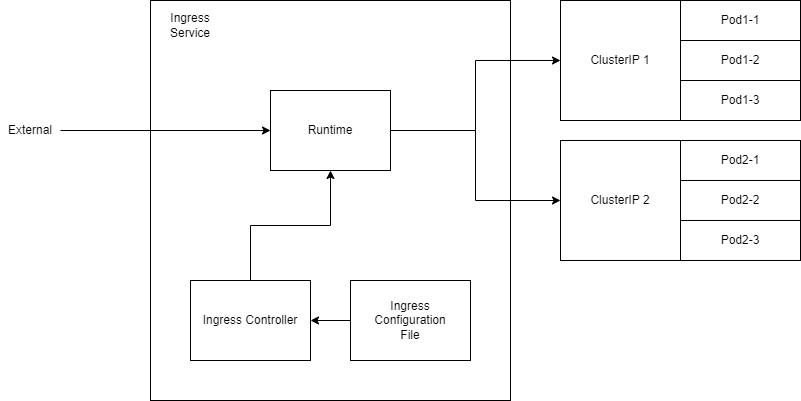
\includegraphics[width=350pt]{chapters/part-3/figures/ingress_service.png}
	\caption{An example of ingress service framework.} \label{ch:vac:fig:ingress_service}
\end{figure}

Below is an example of a Ingress object configuration file from \cite{kubernetes2024doc}.
\begin{lstlisting}
apiVersion: networking.k8s.io/v1
kind: Ingress
metadata:
  name: minimal-ingress
  annotations:
    nginx.ingress.kubernetes.io/rewrite-target: /
spec:
  ingressClassName: nginx-example
  rules:
  - http:
      paths:
      - path: /testpath
        pathType: Prefix
        backend:
          service:
            name: test
            port:
              number: 80
\end{lstlisting}

\section{Kubernetes Cloud Deployment}

Many cloud service providers provide support for Kubernetes deployment. Recall from earlier that AWS supports ECS as the default managed container service. While being very powerful and flexible, the problem with ECS is that it is difficult to migrate across platforms because ECS is proprietary. Once ECS is used, the application is tied to AWS unless the user wishes to setup the configurations all over again on other platforms.

AWS EKS, on the other hand, allows the user to deploy a Kubernetes-based cluster using AWS resources. It allows more flexible migration of the cluster across different platforms. The Kubernetes cluster created and managed by EKS is known as a EKS cluster.

\subsection{Setup and Connect to EKS Cluster} \label{subsec:setupeks}

The following has to be configured when setting up EKS.

\begin{itemize}
  \item Select Kubernetes version.
  \item Select cluster service role which tells AWS resources the EKS cluster can access, such as database, EC2, Container Registry, etc. 
  \item Configure AWS \myabb{Virtual Private Cloud}{VPC}, the AWS network service.
  \item Configure logging.
\end{itemize}

Make sure that AWS CLI is installed on the local machine. Login to the AWS account from the AWS CLI. Once the EKS cluster is setup and active, the user can modify the \verb|kubectl| configuration file which can be found at \texttt{~/.kube/config} so that it points to the EKS cluster. This can be done using AWS CLI as follows.
\begin{lstlisting}
$ aws eks update-kubeconfig --region <region name> --name <eks cluster name>
\end{lstlisting}
With the above, \verb|kubectl| will talk to the EKS cluster but not the local Kubernetes clusters such as the one in Minikube.

\subsection{Configure Node Group}

In the AWS dashboard under the EKS cluster just created, the user needs to configure nodes by adding node groups. This includes at least the following setups.
\begin{itemize}
  \item Attach roles to the node group, for example, to allow nodes to use AWS \myabb{Elastic Compute Cloud}{EC2} and Container Registry.
  \item Select OS for the nodes.
  \item Select EC2 instance type and disk size which will be configured for the nodes.
  \item Select minimum and maximum number of nodes.
  \item Configure AWS VPC for the nodes.
\end{itemize}

It can be seen from the above that node configuration is essentially EC2 configuration. Once these EC2 instances are started, the user can view there status from the AWS dashboard under EC2. However, these EC2 instances shall be managed by EKS entirely and the user should not login to them. EKS should install Kubernetes components upon starting these EC2 instances.

\subsection{Apply Kubernetes Configuration Files}

The Kubernetes configuration files does not need to be uploaded to the cloud. The user can use \verb|kubectl| to apply the configurations to the EKS cluster. Notice that \verb|kubectl| should link to the EKS cluster but not a local Kubernetes cluster such as Minikube. The configuration of \verb|kubectl| to link to the EKS cluster has been introduced earlier in Section \ref{subsec:setupeks}.

At this stage, AWS container registry has not been enabled, so make sure that all the images used in the EKS cluster are from Docker Hub.

\subsection{Use Volumes}

Volumes such as emptyDir and hostPath have been introduced in earlier Sections \ref{subsec:ephemeral_volume} and \ref{subsec:persistentvolume}. They are not useful in the context of EKS cluster.Volume type emptyDir is ephemeral and tied with a Pod, and it is not much useful with the EKS cluster in the production environment where Pods can get started and removed frequently. Volume hostPath can only apply to single node applications which is often not the case with EKS cluster.

With EKS cluster, it is more common to use AWS storage such as EBS, EFS to persist data. CSI is used to link EKS cluster with those storages. PVC is used in the Kubernetes configuration files to claim storage for the applications.

Details of attaching the third-party storage systems such as EFS to Kubernetes services such as EKS are not introduced in details here mainly because the procedures differ from platform to platform. The user should check the user manual for the specific service he wants to use. In general, the user needs to do the following:
\begin{itemize}
  \item Create the storage system with the cloud service provider.
  \item Configure firewall settings and security groups so that the Kubernetes cluster can reach the storage system.
  \item Install necessary drives locally so that \verb|kubectl| supports the storage system related functions.
  \item Create a PV object with a Kubernetes configuration file. Include the storage system specifications such as IP address and drivers in the configuration file, usually under \texttt{spec.csi}. More details are given in \cite{kubernetes2024doc}.
  \item Create a PVC object corresponding with the PV.
\end{itemize}
With the above been done, the EKS cluster objects can use the PVC to persist data.

\section{Kubernetes IDE and Alternatives}

While powerful, Kubernetes and \verb|kubectl| CLI are not beginner friendly. The followings are possible to tackle this issue.
\begin{itemize}
  \item User Kubernetes IDE, which provides a more user-friendly Kubernetes control graphical interface. Examples include LENS \cite{lens2025homepace}. 
  \item User alternative container orchestration tools which are often less flexible and complicated but more user-friendly.
\end{itemize}

Portainer is an open-source container orchestrator that has a user-friendly interface and is relatively easier to use than the more powerful and famous container orchestrator Kubernetes which is introduced in the next chapter. In this section, it is used as an example, just to give the reader an idea what container orchestrators in the market may look like. The section does not go into details about Portainer.

Before starting a Portainer container, it is a good practice to first create a docker volume for Portainer to store the database. Use the following command to create such docker volume.
\begin{lstlisting}
$ docker volume create portainer_data
\end{lstlisting}
Then run a Portainer container using
\begin{lstlisting}
$ docker run -d -p 8000:8000 -p 9000:9000 -p 9443:9443 --name portainer --restart=always -v /var/run/docker.sock:/var/run/docker.sock -v portainer_data:/data portainer/portainer-ce
\end{lstlisting}
where ports 8000, 9000 and 9443 are used for hosting HTTP traffic in development environments, hosting web interface, and hosting HTTPS or SSL-secured services, respectively. The \verb|docker.sock| is the socket that enables the docker server-side daemon to communicate with its command-line interface. The image name for Portainer community edition (distinguished form the business edition) is \verb|portainer/portainer-ce|.

Use \verb|https://localhost:9443| to login to the container. The following page in Fig. \ref{ch:vac:fig:portainerlogin} should pop up in the first-time login, asking the user to create and administration user.
\begin{figure}[!htb]
	\centering
	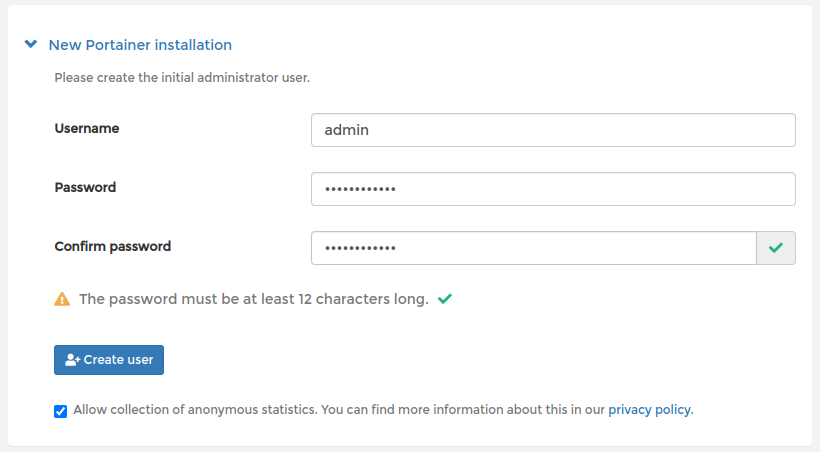
\includegraphics[width=350pt]{chapters/part-3/figures/portainerlogin.png}
	\caption{Portainer login page to create admin user.} \label{ch:vac:fig:portainerlogin}
\end{figure}

After creating the admin user and logging in, the status of images, containers and many more can be monitored via the dashboard, as shown in Figs. \ref{ch:vac:fig:portainerdashboard1}, \ref{ch:vac:fig:portainerdashboard2} and \ref{ch:vac:fig:portainerdashboard3}. Notice that in Fig. \ref{ch:vac:fig:portainerdashboard3}, using the ``quick action'' buttons, the user can check the specifics of the container and interact with its console, just like using \verb|docker container inspect| and \verb|docker exec|.
\begin{figure}[!htb]
	\centering
	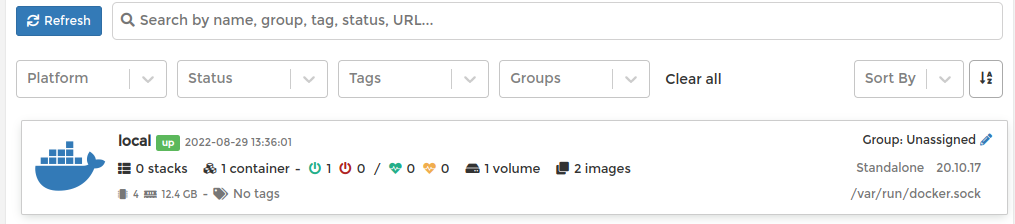
\includegraphics[width=350pt]{chapters/part-3/figures/portainerdashboard1.png}
	\caption{Portainer dashboard overview of docker servers.} \label{ch:vac:fig:portainerdashboard1}
\end{figure}

\begin{figure}[!htb]
	\centering
	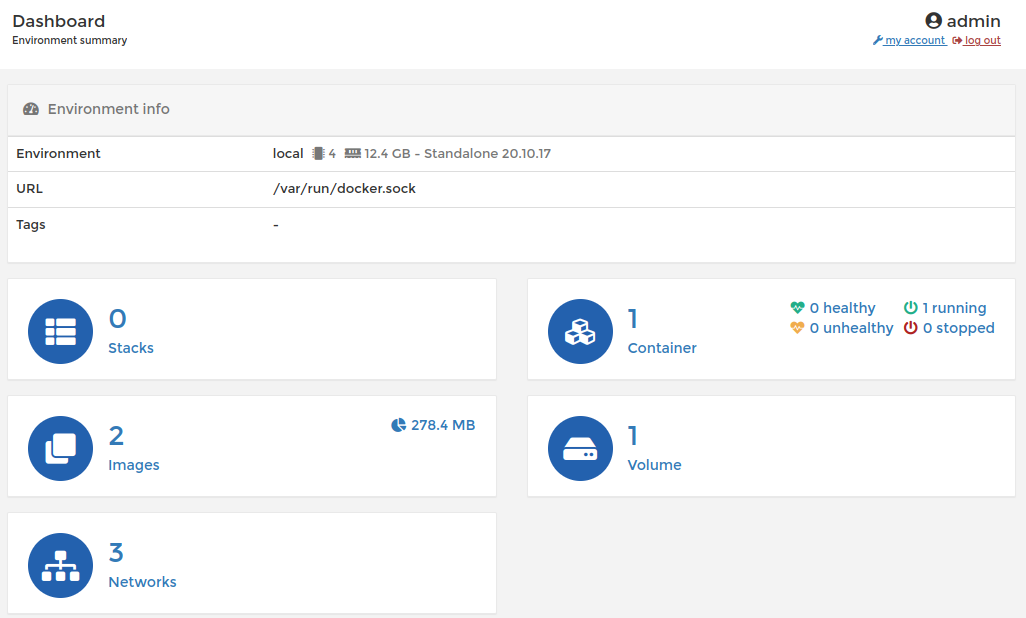
\includegraphics[width=350pt]{chapters/part-3/figures/portainerdashboard2.png}
	\caption{Portainer dashboard overview in a docker server.} \label{ch:vac:fig:portainerdashboard2}
\end{figure}

\begin{figure}[!htb]
	\centering
	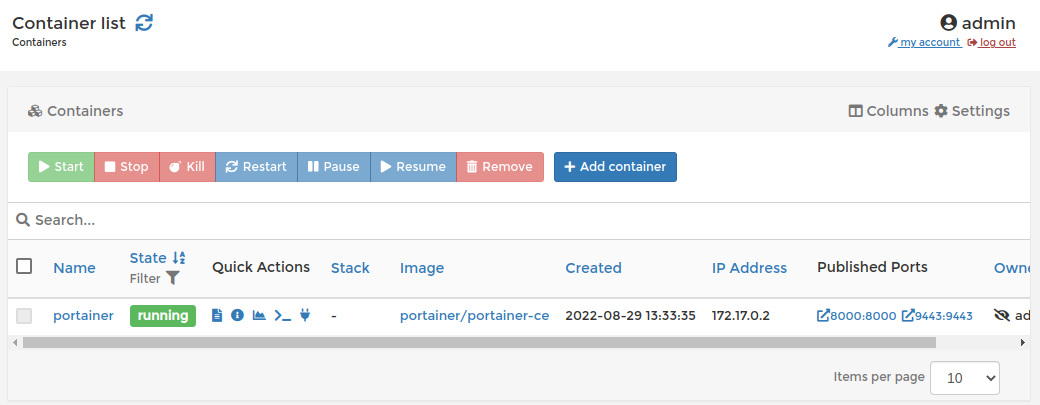
\includegraphics[width=350pt]{chapters/part-3/figures/portainerdashboard3.png}
	\caption{Portainer dashboard list down of all running containers.} \label{ch:vac:fig:portainerdashboard3}
\end{figure}

In summary, Portainer is an easy-to-use container management tool with clean graphical interface that a user can quickly get used to without a steep learning curve. 